\documentclass{beamer}

%% Juego de caracteres usado en el archivo fuente: UTF-8
\usepackage{ucs}
\usepackage[utf8x]{inputenc}
\uselanguage{spanish}
%Para la identación del español
\usepackage[spanish]{babel}

% There are many different themes available for Beamer. A comprehensive
% list with examples is given here:
% http://deic.uab.es/~iblanes/beamer_gallery/index_by_theme.html
% You can uncomment the themes below if you would like to use a different
% one:
%\usetheme{AnnArbor}
%\usetheme{Antibes}
%\usetheme{Bergen}
%\usetheme{Berkeley}
%\usetheme{Berlin}
%\usetheme{Boadilla}
%\usetheme{boxes}
%\usetheme{CambridgeUS}
%\usetheme{Copenhagen}
%\usetheme{Darmstadt}
%\usetheme{default}
%\usetheme{Frankfurt}
%\usetheme{Goettingen}
%\usetheme{Hannover}
%\usetheme{Ilmenau}
%\usetheme{JuanLesPins}
%\usetheme{Luebeck}
\usetheme{Madrid}
%\usetheme{Malmoe}
%\usetheme{Marburg}
%\usetheme{Montpellier}
%\usetheme{PaloAlto}
%\usetheme{Pittsburgh}
%\usetheme{Rochester}
%\usetheme{Singapore}
%\usetheme{Szeged}
%\usetheme{Warsaw}

%Para la identación del español
\usepackage[spanish]{babel}

\title{Success factors in offshoring}

% A subtitle is optional and this may be deleted
%\subtitle{Optional Subtitle}

\author{Jesús Rodríguez Heras: jesus.rodriguezheras@alum.uca.es \\ Alejandro Rosado Pérez: alejandro.rosadoperez@alum.uca.es \\  Gabriel Fernando Sánchez Reina: gabriel.sanchezreina@alum.uca.es \\ Juan Pedro Rodríguez Gracia: juanpedro.rodriguezgracia@alum.uca.es}
% - Give the names in the same order as the appear in the paper.
% - Use the \inst{?} command only if the authors have different
%   affiliation.

%\institute[Escuela Superior de Ingeniería] % (optional, but mostly needed)
%{
%  \inst{1}%
%  Department of Computer Science\\
%  University of Somewhere
%  \and
%  \inst{2}%
%  Department of Theoretical Philosophy\\
%  University of Elsewhere}
% - Use the \inst command only if there are several affiliations.
% - Keep it simple, no one is interested in your street address.

%\date{Vulnerabilidades en redes}
% - Either use conference name or its abbreviation.
% - Not really informative to the audience, more for people (including
%   yourself) who are reading the slides online

%\subject{Theoretical Computer Science}
% This is only inserted into the PDF information catalog. Can be left
% out. 

% If you have a file called "university-logo-filename.xxx", where xxx
% is a graphic format that can be processed by latex or pdflatex,
% resp., then you can add a logo as follows:

% pgfdeclareimage[height=0.5cm]{university-logo}{university-logo-filename}
% \logo{\pgfuseimage{university-logo}}

% Delete this, if you do not want the table of contents to pop up at
% the beginning of each subsection:
%\AtBeginSubsection[]
%{
%  \begin{frame}<beamer>{Índice}
%    \tableofcontents[currentsection,currentsubsection]
%  \end{frame}
%}

% Let's get started
\begin{document}

\begin{frame}
  \titlepage
%  \begin{center}
%  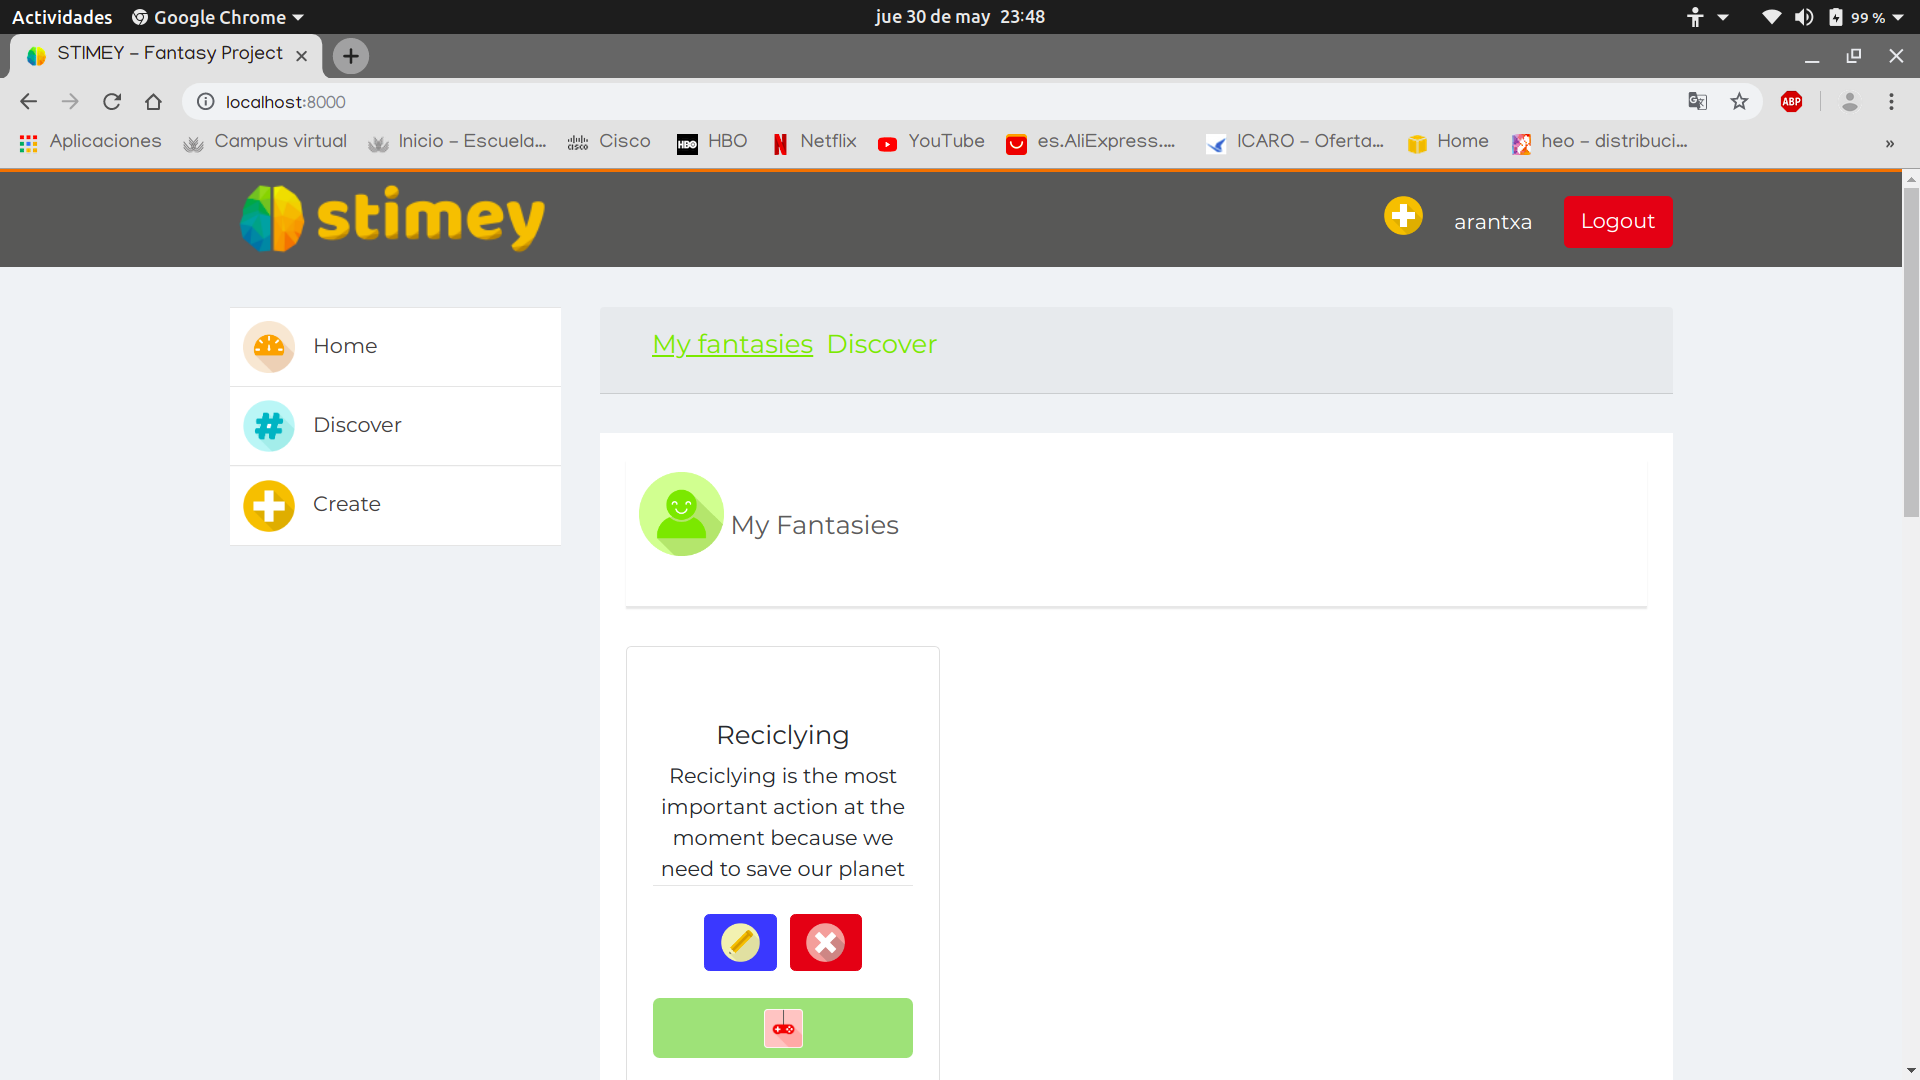
\includegraphics[scale=0.2]{Portada.png}	
%  \end{center}
  
\end{frame}

%\begin{frame}{Índice}
%  \tableofcontents
%  % You might wish to add the option [pausesections]
%\end{frame}

% Section and subsections will appear in the presentation overview
% and table of contents.

\section{A good exapmle: Ketera}
\begin{frame}{A good example: Ketera}
	Ketera is a company that offers software as a service that moved all its functional infrastructure to India since it was cheaper. With this, he was able to offer his services faster and at a lower cost.\\
	\color{white}.\\
	\color{black}
	He currently has a large part of his company there and continues to grow.\\
	\color{white}.\\
	\color{black}
	The key:
	\begin{itemize}
		\item Challenging work.
		\item A great working environment; a place where it’s fun to work.
		\item Open and frequent communications with all levels of management.
		\item Fair treatment.
		\item Opportunity for US travel.
		\item Continuing improvement of technical and soft skills.
	\end{itemize}
\end{frame}

\section{Factors}
\begin{frame}{Factors}
\begin{itemize}
	\item When establishing business relationships, we cannot expect to find a company that is dedicated exactly to what we want.\\
	
	\item The main idea is to conduct an interview with a company and reach a common agreement on how to work together.\\
	
	\item The communication between the employees of the company and those of the other company is crucial for coordination.\\
	
	\item We also need to consider the different lifestyles and attrition of the employees from those places.
\end{itemize}
\end{frame}

\section{Legal problems}
\begin{frame}{Legal problems}
	\begin{itemize}
		\item The differences between the laws of both places must be taken into account.\\
		
		\item In this article, the company hired an external company to manage the entire legal issue.
	\end{itemize}
\end{frame}

\section{How to choose the place?}
\begin{frame}{How to choose the place?}
	When it's time to choose the place of our offshore we need to take care all of those factors:
	\begin{itemize}
		
		\item Overall skills: Its necessary to take care of the employees we hire and their abilities.
		%puntito
		\item Infrastructure: We need to have a look on how good are the local infrastructures; spcially on telecom and costs.
		%puntito
		\item City attraction: Another point is to know how is the quality of life on that place or even how good is the climate or transports.
		%puntito 
		\item Others: Finally we have to keep in mind the fact that vendor interaction has to be good in order to cooperate and succeed.
	\end{itemize}
\end{frame}

\section{Beneffits of offshoring}
\begin{frame}{Beneffits of offshoring}
	\begin{itemize}
		\item Scalability: With offshoring we can request a greater service without worrying about how to reach that demand.

		\item Low cost: offshoring to a developing country allows us to reduce costs, from infrastructure to salary.
		
		\item Greater flexibility: They are able to renegociate with the vendors.
	\end{itemize}
\end{frame}

\section{Summary}
\begin{frame}{Summary}
	The main point to succeed in offshoring is knowing the place and the local people because it makes you choose better.\\
	\color{white}.\\
	\color{black}
	In addition, to get the work well done, it's to maintain a good communication. It makes you able to abstract from de distance and work as a team.
\end{frame}

\end{document}


